\section{Tipos de sensores}
\textbf{Por posición:}

\textbf{Encoder Incremental:} Este tipo de sensor óptico digital convierte el movimiento en una secuencia de pulsos digitales. Tiene una escala transparente con una retícula opaca; de un lado, tiene una escala equipada con una fuente de luz y un lente condensador. Del otro lado, hay celdas sensibles a la luz. La manera en la que funciona es que la resistencia de las celdas disminuye cada vez que reciben un rayo de luz, de este modo se genera un pulso cada vez que un rayo de luz es atravesado.\autoref{fig:20150317193931229}



\begin{figure}[h]
	\centering
	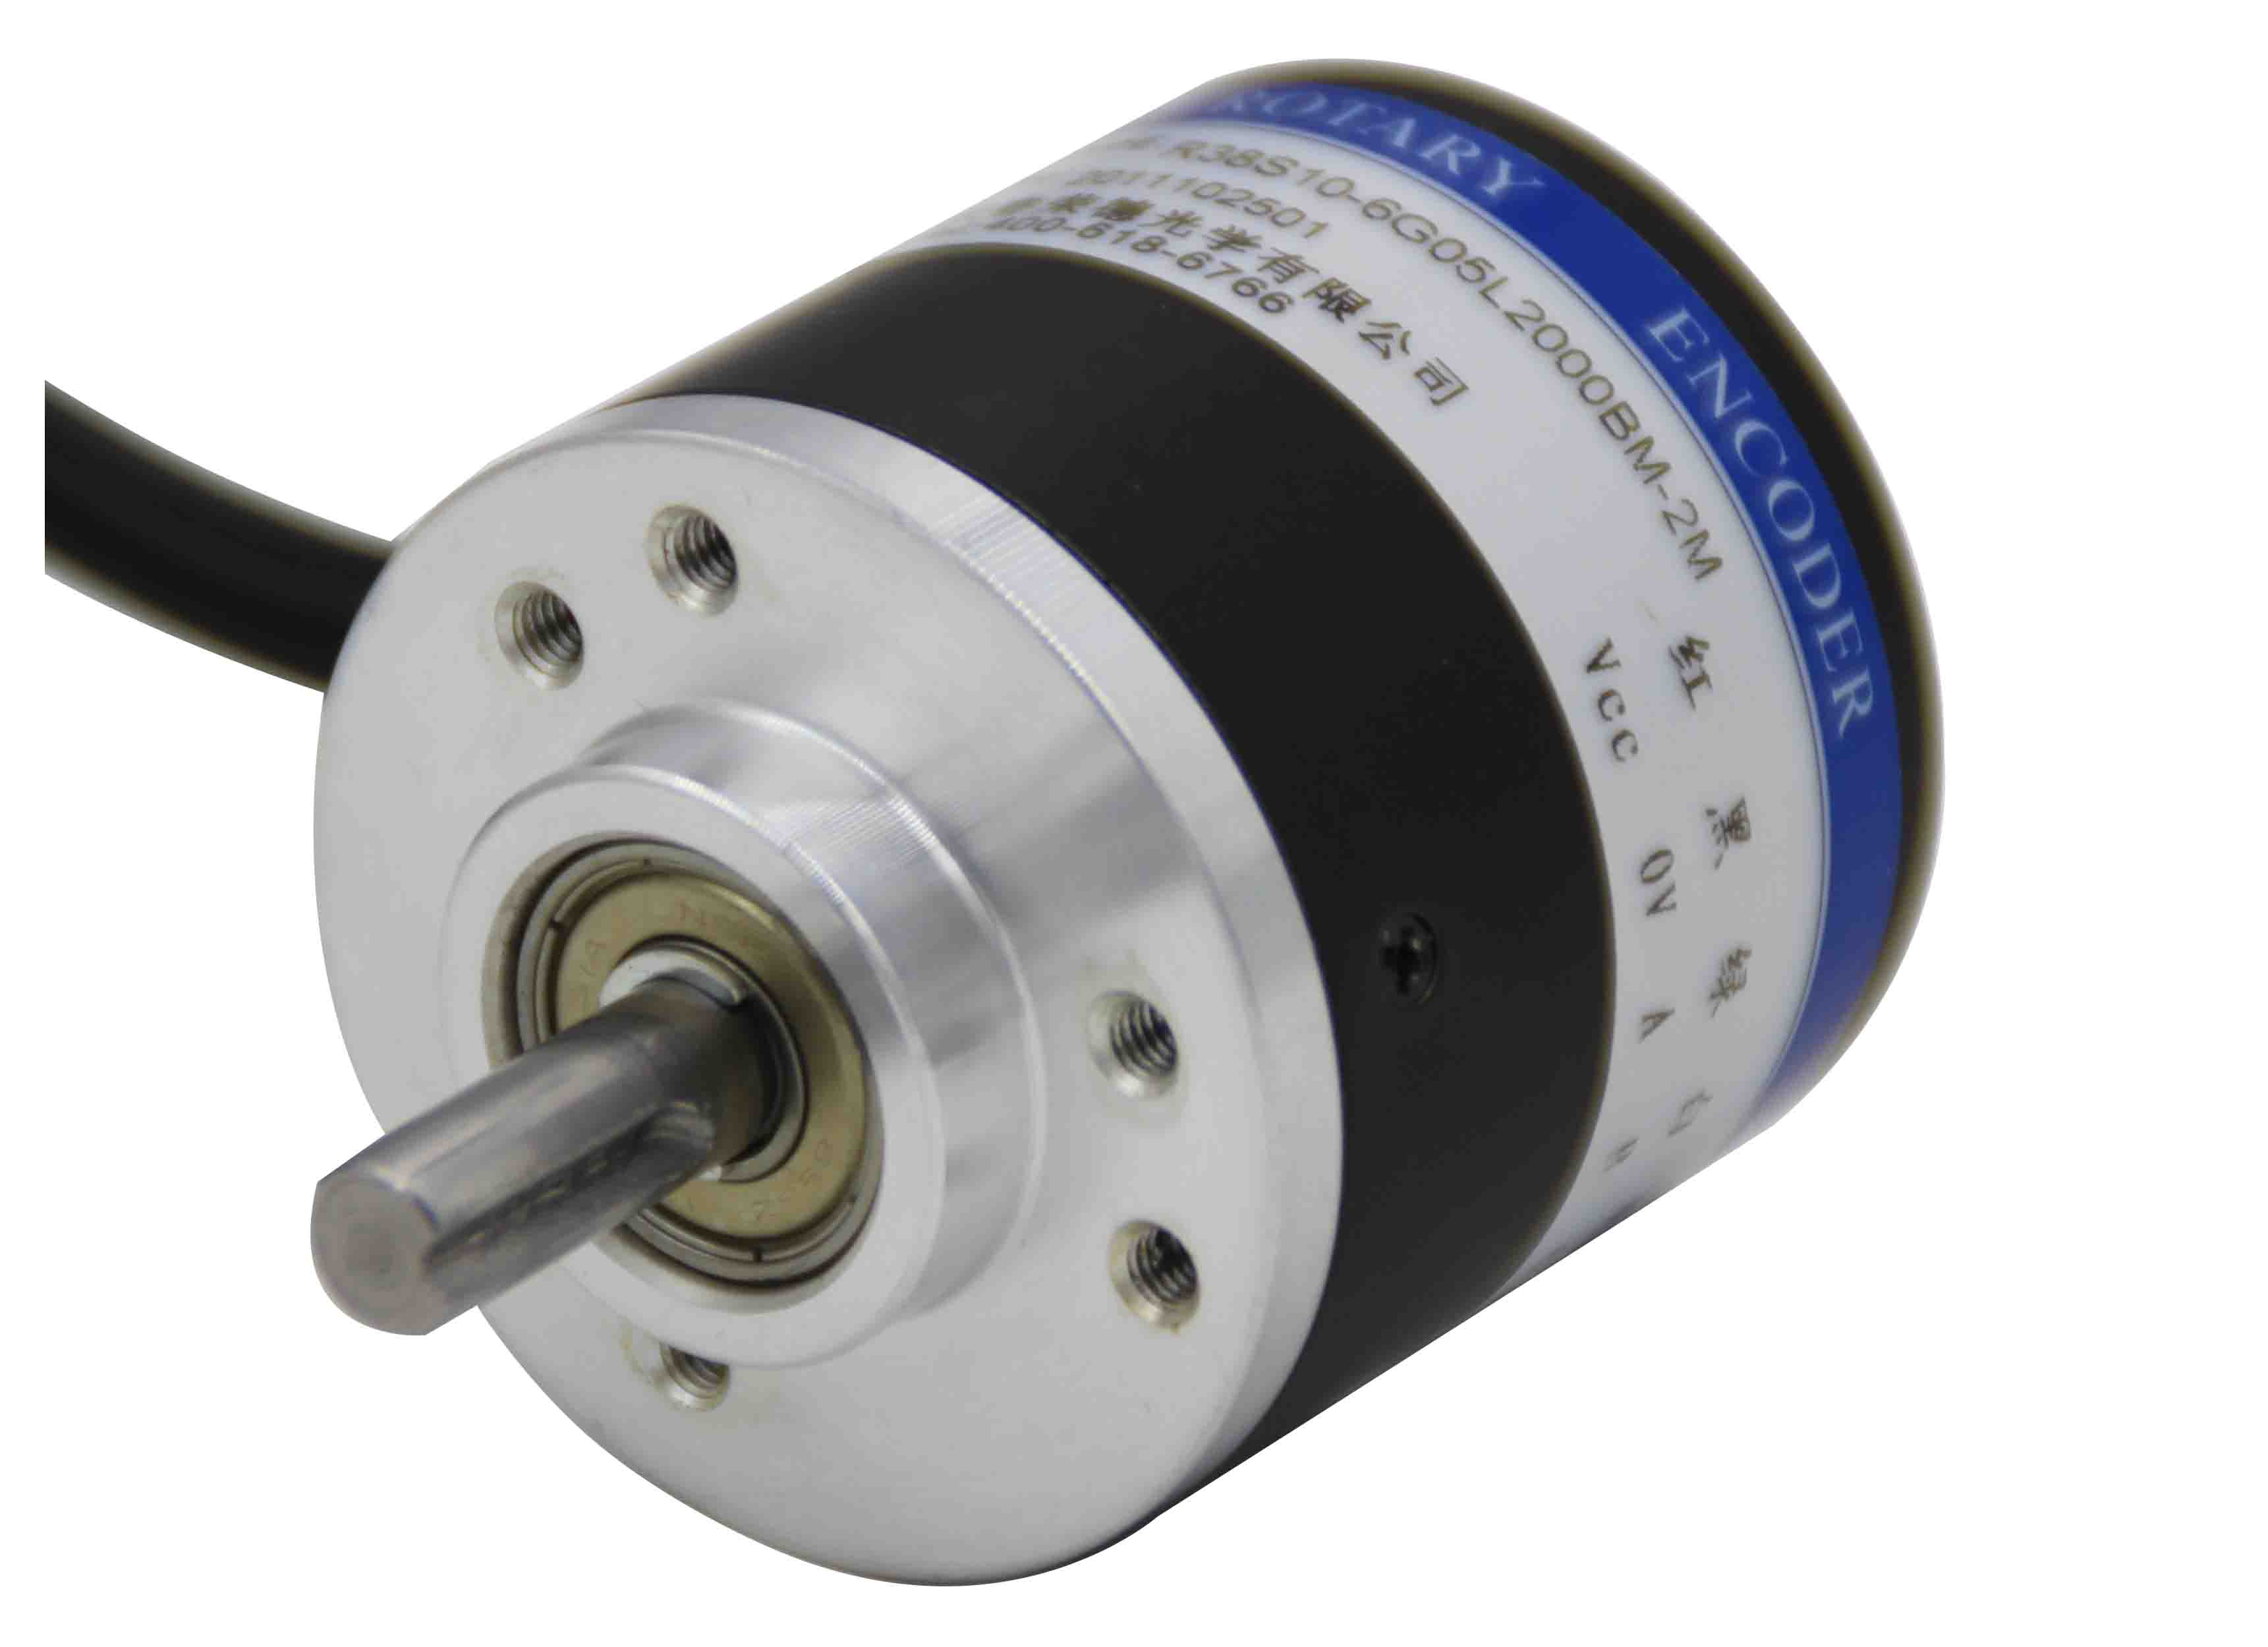
\includegraphics[width=0.4\linewidth]{portada/20150317193931229}
	\caption{}
	\label{fig:20150317193931229}
\end{figure}



\textbf{Potenciómetro:} Es un dispositivo de resistencia variable que expresa desplazamientos lineales o angulares en términos de voltaje. Consiste en una clavija deslizante que hace contacto con un elemento resistivo, conforme se mueve este punto de contacto la resistencia entre el contacto deslizante y las conexiones de los extremos del dispositivos cambia en proporción al desplazamiento. \autoref{fig:potenciometro}\\

\begin{figure}[h]
	\centering
	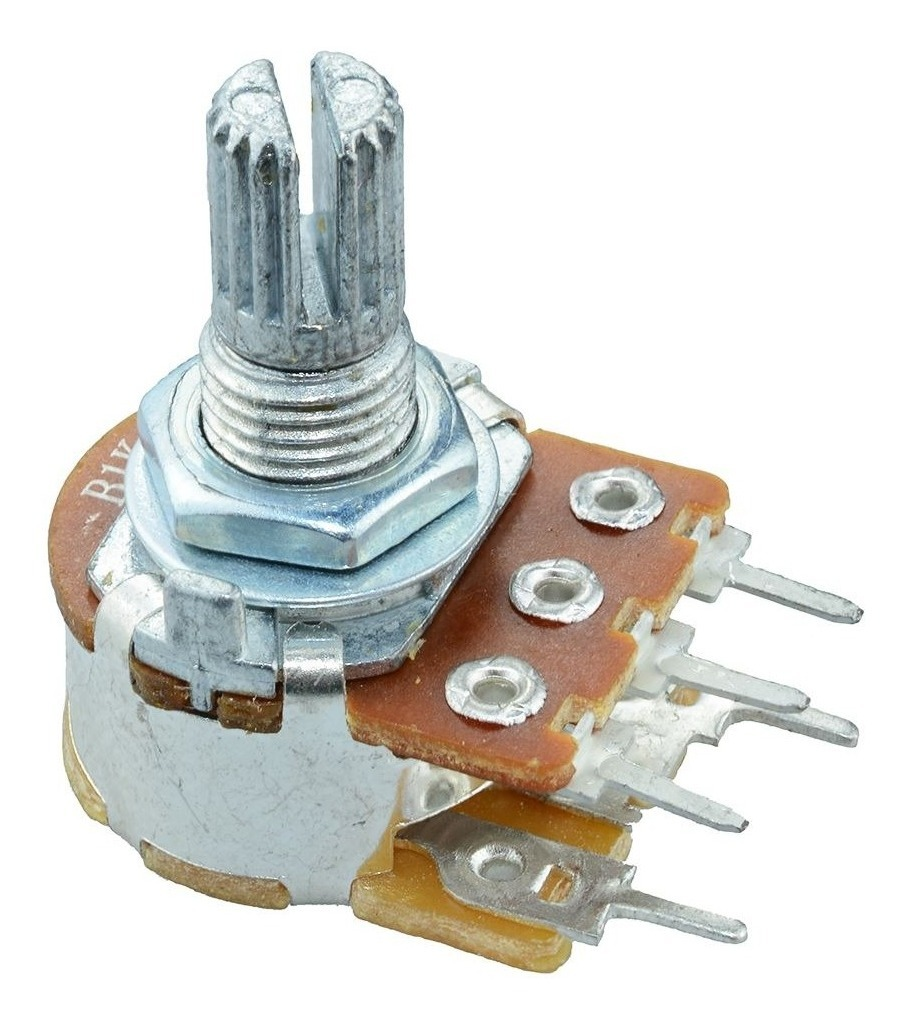
\includegraphics[width=0.2\linewidth, height=0.2\textheight]{img/potenciometro}
	\caption[Potenciómetro]{}
	\label{fig:potenciometro}
\end{figure}



\textbf{LVDT:} Es uno de los transductores de desplazamiento más populares ya que genera una señal de CA cuya magnitud se relaciona con el desplazamiento de un núcleo móvil. Tiene como concepto básico de un núcleo móvil rodeado por dos bobinas secundarias y una bobina principal y conforme el núcleo cambia su posición con respecto a las bobinas cambia también el campo magnético y por tanto se modifica la amplitud de voltaje en la bobina secundaria como una función del desplazamiento del núcleo a través de un segmento considerable.\autoref{fig:lvdt} \\


\begin{figure}[h]
	\centering
	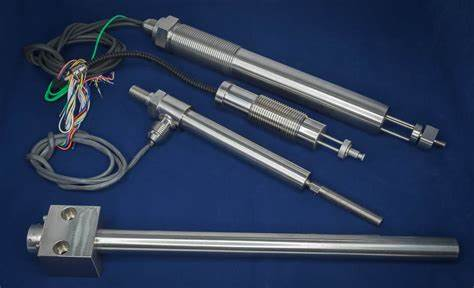
\includegraphics[width=0.2\linewidth, height=0.2\textheight]{img/LVDT}
	\caption{}
	\label{fig:lvdt}
\end{figure}

\begin{figure}[h]
	\centering
	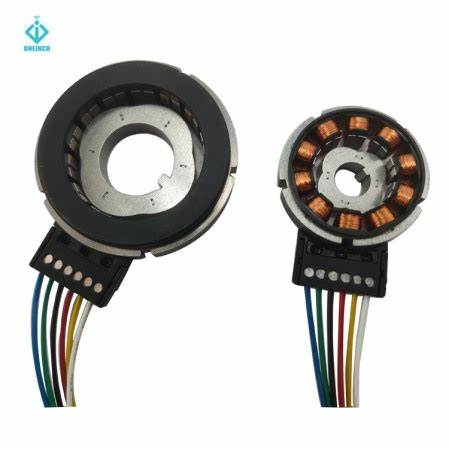
\includegraphics[width=0.2
	\linewidth, height=0.2\textheight]{img/resolver}
	\caption{}
	\label{fig:resolver}
\end{figure}


\textbf{Resolver:} Son sensores que proporcionan señales análogas como salidas y consisten en un eje (flecha) giratoria (rotor) y una carcasa estacionaria. Sus señales tienen que convertirse a la forma digital por medio de un convertidor analógico a digital. Los resólvers tienen dos devanados orientados a 90°. \autoref{fig:resolver}





